\newcommand{\layerheight}{2};
\newcommand{\neuronwidth}{1.5};
\newcommand{\neuron}[3]{\draw[fill, white] (#1 * \neuronwidth, #2 * \layerheight) circle (0.5); \draw (#1 * \neuronwidth, #2 * \layerheight) circle (0.5) node {#3};}
\newcommand{\neuronconn}[4]{\draw (#1 * \neuronwidth, #2 * \layerheight) -- (#3 * \neuronwidth, #4 * \layerheight);}
\newcommand{\neuronconnst}[5]{\draw[#5] (#1 * \neuronwidth, #2 * \layerheight) -- (#3 * \neuronwidth, #4 * \layerheight);}

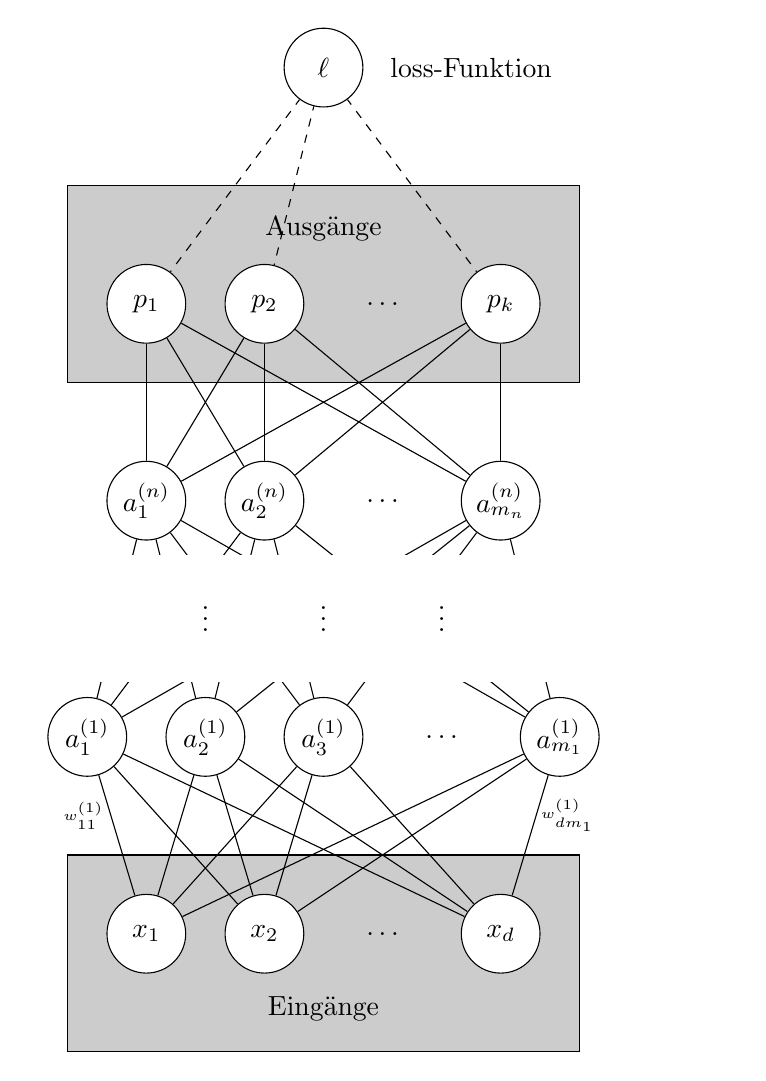
\begin{tikzpicture}
	\draw[fill=black!20] (-1, -1.5) rectangle (5.5, 1) node[midway, yshift=-20] {Eingänge};
	\draw[fill=black!20] (-1, 7 / 2 * \layerheight) rectangle (5.5, 9.5 / 2 * \layerheight) node[midway, yshift=20] {Ausgänge};

	% Verbindungen
	\neuronconn{0}{0}{-0.5}{1.25}
	\neuronconn{0}{0}{0.5}{1.25}
	\neuronconn{0}{0}{1.5}{1.25}
	\neuronconn{0}{0}{3.5}{1.25}
	\neuronconn{1}{0}{-0.5}{1.25}
	\neuronconn{1}{0}{0.5}{1.25}
	\neuronconn{1}{0}{1.5}{1.25}
	\neuronconn{1}{0}{3.5}{1.25}
	\neuronconn{3}{0}{-0.5}{1.25}
	\neuronconn{3}{0}{0.5}{1.25}
	\neuronconn{3}{0}{1.5}{1.25}
	\neuronconn{3}{0}{3.5}{1.25}
	
	\neuronconn{-0.5}{1.25}{0}{2.75}
	\neuronconn{-0.5}{1.25}{1}{2.75}
	\neuronconn{-0.5}{1.25}{3}{2.75}
	\neuronconn{0.5}{1.25}{0}{2.75}
	\neuronconn{0.5}{1.25}{1}{2.75}
	\neuronconn{0.5}{1.25}{3}{2.75}
	\neuronconn{1.5}{1.25}{0}{2.75}
	\neuronconn{1.5}{1.25}{1}{2.75}
	\neuronconn{1.5}{1.25}{3}{2.75}
	\neuronconn{3.5}{1.25}{0}{2.75}
	\neuronconn{3.5}{1.25}{1}{2.75}
	\neuronconn{3.5}{1.25}{3}{2.75}
	
	\neuronconn{0}{2.75}{0}{4}
	\neuronconn{0}{2.75}{1}{4}
	\neuronconn{0}{2.75}{3}{4}
	\neuronconn{1}{2.75}{0}{4}
	\neuronconn{1}{2.75}{1}{4}
	\neuronconn{1}{2.75}{3}{4}
	\neuronconn{3}{2.75}{0}{4}
	\neuronconn{3}{2.75}{1}{4}
	\neuronconn{3}{2.75}{3}{4}
	
	\neuronconnst{0}{4}{1.5}{5.5}{dashed}
	\neuronconnst{1}{4}{1.5}{5.5}{dashed}
	\neuronconnst{3}{4}{1.5}{5.5}{dashed}
	
	% Eingänge
	\neuron{0}{0}{$x_1$}
	\neuron{1}{0}{$x_2$}
	\draw (2 * \neuronwidth, 0 * \layerheight) node {$\dots$};
	\neuron{3}{0}{$x_d$}
	
	% 1. Layer
	\neuron{-0.5}{1.25}{$a_1^{(1)}$}
	\neuron{0.5}{1.25}{$a_2^{(1)}$}
	\neuron{1.5}{1.25}{$a_3^{(1)}$}
	\draw (2.5 * \neuronwidth, 1.25 * \layerheight) node {$\dots$};
	\neuron{3.5}{1.25}{$a_{m_1}^{(1)}$}
	
	\draw[fill, white] (-1 * \neuronwidth, 1.6 * \layerheight) rectangle (5 * \neuronwidth, 2.4 * \layerheight);
	\draw (3 / 2 * \neuronwidth, 2 * \layerheight + 0.1) node {$\vdots$};
	\draw (1 / 2 * \neuronwidth, 2 * \layerheight + 0.1) node {$\vdots$};
	\draw (5 / 2 * \neuronwidth, 2 * \layerheight + 0.1) node {$\vdots$};
	
	% n. Layer
	\neuron{0}{2.75}{$a_1^{(n)}$}
	\neuron{1}{2.75}{$a_2^{(n)}$}
	\draw (2 * \neuronwidth, 2.75 * \layerheight) node {$\dots$};
	\neuron{3}{2.75}{$a_{m_n}^{(n)}$}
	
	% Ausgänge
	\neuron{0}{4}{$p_1$}
	\neuron{1}{4}{$p_2$}
	\draw (2 * \neuronwidth, 4 * \layerheight) node {$\dots$};
	\neuron{3}{4}{$p_k$}
	
	% Training
	\neuron{1.5}{5.5}{$\ell$}
	\draw (1.5 * \neuronwidth +1.25 * \neuronwidth, 5.5 * \layerheight) node {loss-Funktion};
	
	\draw (-0.80,1.5) node[font=\tiny] {$w_{11}^{(1)}$};
	\draw (5.35,1.5) node[font=\tiny] {$w_{dm_1}^{(1)}$};
\end{tikzpicture}